\chapter{Implementation}\label{cha:implementation}
The following chapter documents the different functional modules that were implemented according to the proposal. 
Most of them interact with each other through the DSMs, which has been added as well as a module for its 
understanding.

\section{LED Control}\label{sec:leds}
*Redaction style at 95/100

In order to notify to the user the current state of each axis, the robot includes one or more LED rings. These rings are 
 a serial array of LEDs that are programmed and controlled through a serial communication protocol. Basically, the final implementation
 is an adaptation of a library that uses a PWM peripheral to generate a signal that is modulated according to the data that 
 controls the LEDs, namely digital 1s, 0s and reset as a specific duty cycle. The input pin of the first LED is connected to the MCU and depending on the modulated data, it will be 
 passed over the next LEDs, being the first LED's output the input of the next til the last component. A summary of the 
 protocol is explained in ~\cite{led_protocol}. 

 In the next paragraphs a summary of the activities that were carried out during the implementation is presented.

\begin{description}
\item[First control tests] Learning the basics of the interface used to control one LED
\item[Code for one LED control] Using the peripherals of the MCU simple routines were written to set different basic colors in RGB. 
    The peripheral used were a two Timers (hardware libraries) to keep control of the data timing and refresh rate.
\item[Search for libraries] Once the basic communication was understood, it was clear that the usage of libraries would be more practical,
    since the first approach were not suitable for higher number of LEDs and effects; moreover, the CPU was kept busy while waiting 
    the timer state polling. The libraries found were aiming roughly either 8/16 bits processors whose main task was controlling the LEDs, 
    or more complex libraries that used DMA modules within 32-bit processor. One of the latter implemented modulation of the data over a PWM and a
    DMA peripheral for one LED strip.
\item[First library selection] Due to the inexperience working with DMA modules and as the LED control was not of a higher priority compared to other tasks, 
    it was decided to run first one of the basic libraries to achieve a multi LED control. The implementation was able to control a set of 20 LEDs
    with the processor mainly polling the Timer states.
\item[Further control tests] Despite the success of the library with one channel, the overall structure of the basic library
    was not easily portable to the proposed solution using FreeRTOS. Additionally, the DMA libraries showed afterwards being easier 
    to modify as they were designed with a more abstracted and multi-purpose approach.
\item[Second library selection] As the usage of DMA became clearer, it was decided to improve the approach by 
selecting a 32-bit processor based library, that implemented only general control functions to avoid massive code lines
related to effects and other rather unnecessary features, yet structured enough to be easily adapted. 
The final result was based upon the WS2812 Library for STM32F4 from Uwe Becker, see \cite{led_library}. 
    Main modifications were the addition of multiple channels capability and global flags needed for synchronizing with DSMs.
\end{description}


\section{Temperature acquisition}\label{sec:temperature}
*Redaction style at 90/100

Similar to the LED control's library, the temperature readout needed a library to be modified to match the current project.
\begin{description}
\item[First readouts] Working with the temperature sensors was the first task in schedule, so it helped train the basic usage
    of the IDE \emph{STM32Cube}, along with the hardware configuration of the MCU and the HAL libraries. 
    The sensor uses a one-wire serial protocol, which similarly to LED Control's first approach was implemented by using 
    timers for controlling 1s and 0s high levels, a continuous polling of data and a general while loop approach. 
    This method worked as intended but it was known from the beginning that it would not match the multi-tasking proposal. 
    However, it was of great importance to get to know the hardware and software, besides more functions were needed to 
    access the sensor's ROM needed e.g. for identification.
\item[FreeRTOS first tests] Short after the working code was used to do the first tests with the RTOS, 
    in this manner the code was translated as a Task (Thread as called by CMSIS) and some features like prioritization, 
    task attributes, task handling and signals were tested with other generic functions, e.g. clocks and PWM generators. 
    However, this implementation was not able to handle multiple one-wire devices due to its absence of CRC comparison.
\item[Integration of library] Finally, it was decided to adapt one open source library designed for STM32 processors. 
    This is based on the principle that UART speeds @9600 and @11200 bps suits the One-Wire timing, such that the 
    detection of One-Wire devices and communication process can be downloaded to hardware already included in many 
    general-purposes processors using USART. The integration of this library is from design compatible with RTOS, 
    namely with CMSIS-RTOS. The library selected was developed by Tilen MAJERLE, review in \cite{temp_library}, and it 
    was barely modified as it contained already the desired functionalities and the development
    focused only on the integration into the DSMs and usage of it. 
\end{description}

The strategy the final library is based on is rather interesting and more details can be read in \cite{onewire_theory}.

\section{EtherCAT Slave communication: SOES adaptation}\label{sec:soes}
*Redaction style at 85/100

This functional module is the one with highest priority, therefore most of the effort given was focused not only 
on the library itself but the protocol and the hardware commissioning. Hence, this section was extended and divided
as follows: first, more technical details are presented regarding the EtherCAT specification, such that the SOES
features are better understood. As to the next subsection, some constraints for the prototype are commented and the 
available hardware is explained*. Once summarized, the main points of the implementeation are presented.

\subsection{EtherCAT data consistency and constraints for design}\label{sec:ecat_sms}
This subsection describes both the features with which the \emph{Axis Communication Board} has compatibility, and a summary of the mechanism that the protocol
implements at the low level to work with the data exchange between Master and Slave. The constraints that were set were part of a live process that ran all along
the learning process of the protocol itself. This is important to mention, since the understanding of the protocol leads to a sinful selection of the features
that a device should have implemented. Therefore, the understing process was a natural consequence from the integration of the SOES library. It is presented however before, such that 
it is understandable what features became priorities and which others are now presented as proposals.

The reader may recall the set of Communication Profiles that are available within the EtherCAT fieldbus, see \ref{sec:ecat_protocol}. From them, the Mailbox and CoE 
are the main features with which the Axis Communication Board works. Leaving aside for future integration the FoE and EoE, the forme would make possible 
update the device by sending a firmware binaries to the device's bootloade; whereas the latter would make the ACB* accessible for any IT tool based on TCP/IP.




\subsection{SOES}
*Redaction style at 90/100

%*Here comes the information about what SOES do, how is the license, what are the features that has already included, the futures that don't, how general it is, an image of its structure, the work that needs to be done*
As briefly commented in section \ref{sec:openness}, the types of licenses allow open development and integration of software. 
SOES software stack was written in C and published based upon the GPLv2, which is a Copyleft License. However, the tools developed 
by the Open EtherCAT Society which support the design, implementation and certification of EtherCAT slaves using the mentioned stack 
are comercial ones. A significant part of the challenge covered by this Project Research was to achieve the EtherCAT Slave functionality
in the prototype without those tools, as the protocols are open.
In table \ref{tbl:soesrequirements} can be seen the main features abstracted and available in the stack, as well as the overall tasks to 
carry out for a device to work properly.


\begin{tuhhtable}
    \begin{tabular}[tp]{L{.3\textwidth}L{.3\textwidth}}
      \THc{1}{c}{Features} &  \THc{1}{c}{Requirements} \\
      \abovebodyrule
        EtherCAT State Machine  & Build up the SII-EEPROM Data-Layout     \\\TRc
        Mailbox Interfaces      & Create the ESI-file     \\
        CoE                     & Port libraries to the STM32 using HAL drivers     \\\TRc
        FoE + bootstrap template& Use FreeRTOS for scheduling (Hardware Requirements $RAM>64KB$)     \\
      \belowbodyrule
    \end{tabular}
    \caption{Features of SOES library and the overall requirements to make it work.}
    \label{tbl:soesrequirements}
  \end{tuhhtable}


\subsection{EtherCAT Slave Controller (ESC): LAN9252} 
As part of the available hardware introduced in \ref{cha:solution}, the LAN9252-EVB-SPI is an evaluation kit for the ASIC LAN9252 manufactured by Microchip. 
This IC is an EtherCAT Slave Controller with 4K bytes of Dual Port memory (DPRAM) and 3 Fieldbus Memory Management Units (FMMUs). 
Each FMMU performs the task of mapping logical addresses to physical addresses.
The EtherCAT slave controller also includes 4 SyncManagers to allow the exchange of data between the EtherCAT master and the local application.[?]%Reference to LAN9252 datasheet 
As briefly summarized in \ref{sec:ecat_sms}, each SMX direction and mode of operation is configured by the EtherCAT master. Two modes of operation 
are available: buffered mode or mailbox mode. 
In the buffered mode, both the local microcontroller and EtherCAT master can write to the device concurrently. The buffer within the LAN9252 
will always contain the latest data. If newer data arrives before the old data can be read out, the old data will be dropped. In mailbox
mode, access to the buffer by the local microcontroller and the EtherCAT master is performed using handshakes, guaranteeing that no data 
will be dropped. The overall structure of the ASIC can be seen in \ref{fig:lan92struct}.

%Which mode is more efficient, what are the advantages and disadvantages?

\fignoframe{imgs/impl-lan-structure_s}{Internal structure of the LAN9252, highlighting the PDI which was selected for this application to be SPI}{fig:lan92struct}

\subsection{Development}
*Redaction style at 70/100
Once explained the general information regarding the Communication Profile, the library and the hardware, the following lines will list and
expose some of the most relevant information during the integration. 

\begin{description}
\item[Porting the low-level functions of the library] THIS
\item[First tests with most basic read funcions over spi] THIS
\item[Selecting the features to be implemented on MCU Host according to specification and complexity] THIS
\item[Second tests with read/write functions for directly addressed registers] THIS
\item[Third tests with the EtherCAT Master] At this stage a compilant EtherCAT Master was configured through a PC running \emph{TwinCAT 3}. In order to ensure a reliable configuration two different EtherCAT devices were connected synchronizing their data with the Master. Namely, a comercial 3-Phase Motor Controller (\emph{ELMO Controller}) and an in-house multi-protocol end effector tool. For those different data structures were declared and very simplistic update loops were programmed within the XAE environment using \emph{SText****} programming language.
\item[Creation of an ESI file and flashing] **Mention that the existing information is either for the Beckhoff's ET1100 or PIC32 (in the case of the LAN9252 set of APIs).
\item[Object dictionary] **Mention that according to the standard *mention the standard for ESI files** and object dictionary was created matching to the one contained in the ESI file, but mapped according to the few documentation available of SOES.
\item[Fourth tests: running the flashed device] Longer tests and configuration loop due to the deepening on EtherCAT protocol. Refer to the the SMs characteristics**** Constant comparisons between the data read by the Master *this could have another image from the mapping access through XAE* and the data received by the MCU host.
\end{description}


\section{Device State Machines (DSMs)}\label{sec:statemachines}
*Redaction style at 85/100
% Guideline
%     Introduction
%     SMS and interaction    
%     Synchronization approach, UPPAAL representation
%     Introduce the SMs what things have to be taken into account for the scheduling and prioritization

In order to have a deterministic behaviour of the embedded system, a set of State Machines (DSM) -not to be confused with Synchronization Manager- were proposed 
and implemented as part of the project library. 
The DSMs software implementation follows a case comparator approach, since it was simple, yet effective and flexible enough, 
to work during the prototype. 
These characteristics were very important, since the DSMs structures were in constant change as the integration of new libraries 
and the functionalities developed. 
The proposed DSMs are as follows and the diagrams can be reviewed in appendix \ref{cha:state_machines}.

\begin{description}
\item[Event Handler] Its purpose is to react to notifications or errors that could appear within other DSMs and notify to update the LED rings in accordance.
                    The approach of having defined this DSM was mainly thought for fault handling and will be the base for the inclusion of future features, e.g.,
                    receiving commands or interruption requests from any of the interfaces. See in \ref{fig:sm_event}.
\item[Temperature] Initializes and runs the temperature related functions. It relies primarily on the open-source library. See in \ref{fig:sm_temp}.
\item[ECAT] Initializes the EtherCAT communication and activates the SOES App. It is important to mention, that this DSM is rather focused on synchronization 
            with the SOES state machine. The latter changed as the development advanced, since the native infinite loop the SOES library is based on had to be adapted.
            The two involved DSMs can be seen in \ref{fig:sm_ecatsoes}.
\item[LED] Initializes and updates periodically the RGB value of the LED Rings. See in \ref{fig:sm_led}.
\end{description}

As to the representation of the DSM, it is important to consider the general two apporaches for Finite State Machines, namely Mealy and Moore, since both 
of them provide advantages while abstracting the desire logic of the different functional blocks. In this rather practical approach the formalities are not fully
met, for instance, to choose strictly for transitions dependent on the state and inputs with actions, but using exit actions as part of each state, when it is convenient.
There are though transitions that explicitly executes a synchronization edge. This flexibility was opted due to the inherent interconnection of the DSMs
as they are not fully independent. To meet a suitable representation, the previously said is integrated with the approach of \emph{UPPAAL} 
software to model timed automata and the reader is invited to look it up in \cite{uppaal_tutorial}.
As a summary, since the modelling of automata for real time systems demands a synchronization feature, this is represented and attached to the edges between 
locations (location in the sense that a state is a location constrained to valuated time and other variables) with the symbols $?$ and $!$, the one* acting as 
a wait action and the latter as a notification. Those, clearly can be understood as signals between different threads.


\subsection{Scheduling}\label{sec:scheduling_intro}
*Redaction style at 85/100
%Guidelines
% introduction
% --------------------
%     Mention the scheduling apporach of RTOS
        
%         List of proposed threads and description of them (only proposal)
%         Priority based, fixed and not based on Execution times
%            >> Time proposed for each one, mention that it is also configurable. 
%           SPI speed calculation?
%         This is a Table
     
% ---------------------This is in results-----------------------------------
%     Problems in the implementation 
%         Priority of each task + timer priority
%             Solutions + Task manager
%          Present the final table of threads
%         explains events its problems with timers, etc    
%             Solutions
%     List of resources that might demand mutex
%             List of general variables
%         Regardinf the synchronization: How the OS prevents from problems?
%             solutions
%           Future improvement (3 items for OS debugging)

In the present section, the main points regarding thread management and scheduling is presented.
All the DSMs were implemented as \emph{Threads} using CMSIS-RTOS on STM32. All threads have fixed priorities and the desired execution time
(\emph{release}) is controlled to each thread through the OS-native delay function. The previously mentioned function is not to be confused 
with the \emph{HAL} version of it, since using HW-related functions while executing an OS is conveniently avoided. The OS-function allows 
the scheduler to allocate CPU resources to any next-priority tasks. For further information regarding HAL and CMSIS implementation of delay
can be seen in [?] and [?]. The time constraints are defined as \emph{desired}, since the system is
non Safety-Critical -recall the safety specifcation in \ref{tbl:tech_specs}-; hence, it has no hard real time constraint and the overall 
execution follows a best effort approach. This, however, opens the door to further improvement in the sense of characterizing and optimizing
the reliability and task execution; the latter will be commented in the results section \ref{sec:scheduling_results}. 

In \ref{tbl:threads_generals} are presented the basic timing requirements depending on the functionalities of each DSM related to the thread.
Each parameter that sets up the duration can be changed in a header file, see the annex header [?], and the individual functionality can be 
reviewed in the previous DSM section, \ref{sec:statemachines}.
%**Here comes a table with the priority for each task**
\begin{tuhhtable}
    \begin{tabular}[tp]{L{.3\textwidth}C{.3\textwidth}}
      \THc{1}{c}{Thread} &  \THc{1}{c}{Release period (ms)} \\
      \abovebodyrule
        SOES APP SDM    & 5 to 10     \\\TRc
        LED SDM         & 33    \\
        ECAT SDM*        & 100     \\\TRc
        Temperature SDM & 1000     \\
      \belowbodyrule
    \end{tabular}
    \caption{Basic timing requirements for threads, deadlines are rather desired since the device is non Safety-Critical. \emph{*ECAT SDM 
        is mainly event driven, nevertheless, in the connected state it has a periodic update}}
    \label{tbl:threads_generals}
  \end{tuhhtable}

A final list of priorities and threads is presented in the table \ref{tbl:threads_final} wihtin the section of Results \ref{sec:results}.

%RAte monotonic oder deadline monotonic???
%EDF ----Scheduling , is this for dynamic priorities?


\section{PCB}
*Redaction style at 90/100


%Guidelines
%   Purpose : to have a prototype
%              Altium design
%               Create a framework for hardware development
%   Based on NUCLEO 
%   Altium 3D design
%  ! Foto of real one 
%       List of issues with a simple solution
%       List of improvements
%   
%   -------------Not necessary
%   Table with, number of layers, size
%   BOM, connectors, pcb specifications
In this section straightforward information regarding the the manufacturing of the PCB proposal is given.
The schematics and PCB layout can be consulted within the appendix \ref{appx:pcb}. The main idea around this design was introduced in 
\ref{sec:pcb_proposal} and has the purpose of providing experience in embedded hardware design and a base work for comming projects, where
the functionalities of this prototype will be merged with other boards. Therefore, to have a physical prototype to recognize
possible opportunity areas, such as physical connectors, sizes, power source quality and signal integrity, is a corner stone for any 
future design.
The overall stages of this design are as follows:
%75/100
\begin{description}
\item[Design] \emph{Altium} PCB design software was used to prototype the PCB for this project. During the process the first approach was
                based on the open files for both the NUCLEO-F446ZE Development Board by ST [?] and LAN9252-EVB-SPI by Microchip[?]. By analizing
                the general diagrams and selecting and adapting the different modules to adapt the requirements was the main challange. To ensure
                usage of less extra devices as possible, two voltage regulators were included for 5 and 3.3 V.
                To meet the routing needs a four layered PCB was selected. The final 3D model can be ssen in figure \ref{fig:pcb3d}
\end{description}

\begin{figure}[ht]
    \centering
    \subfigure[ACB 3D view top]{\label{subfig:pcbtop}{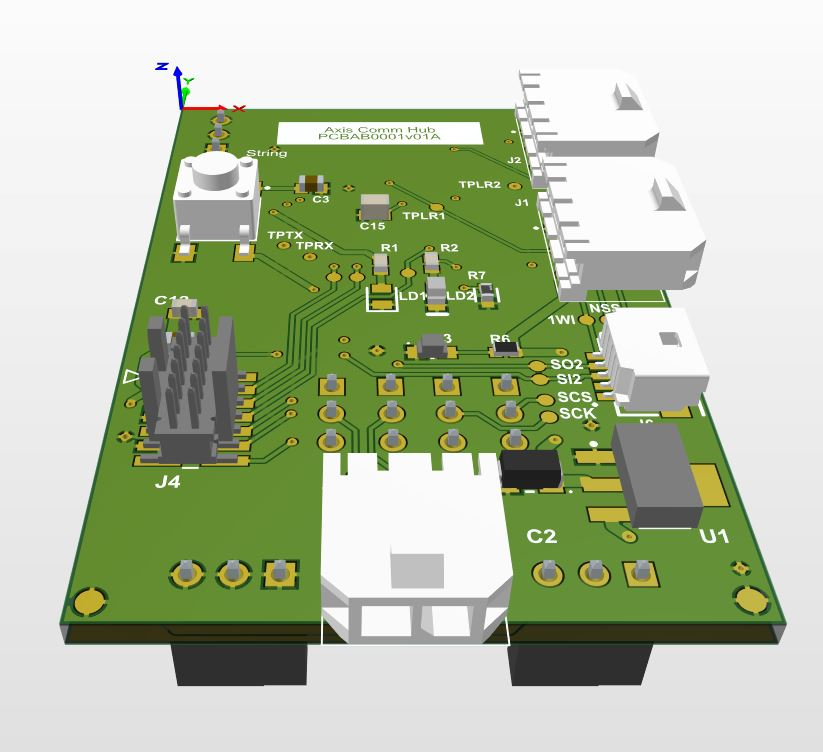
\includegraphics[width=0.4\textwidth]{imgs/pcb3d_1.JPG}}}\hfill
    \subfigure[ACB 3D view bottom]{\label{subfig:pcbbottom}{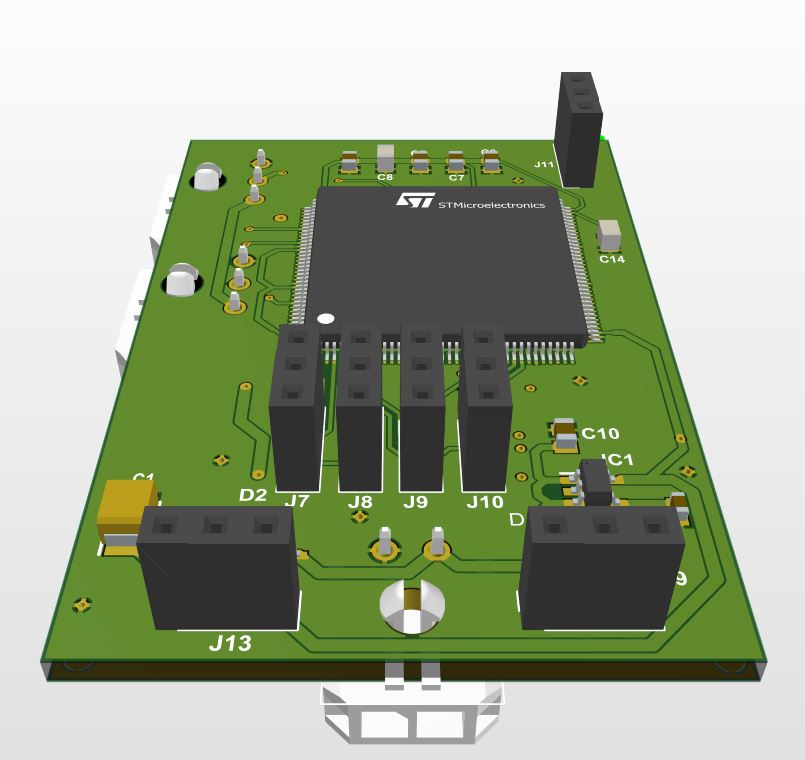
\includegraphics[width=0.4\textwidth]{imgs/pcb3d_2.JPG}}}
    \caption{3D model generated by Altium for the final design.}
    \label{fig:pcb3d}
\end{figure}


\begin{description}
\item[Manufacturing]    Due to practical reasons, the board manufacturing process was in charge of PCBWay, a PCB manufacturing company. In respect
                to soldering, it was made in-house.

\item[Testing I] The overall integrity and functioning of the Power-on and SWD-Programming of the STM32 MCU via SWD/JTAG connector on-board was firstly tested with good results. 
\end{description}

\begin{description}
\item[Testing II] By this stage, the readout of directly addressed memory space, specificaly test and ID register, of the LAN9252 had been already done
                    with the NUCLEO board. In this manner, the code was programmed onto the AXB and so, the SPI communication gave good results*. Moreover,
                    the PWM Outputs over the two channels for WS2812 LED control and the 1-wire connection were also physycally tested.  
\item[Testing III] This phase is an ongoing task, since depending on the development of all the features, communication speeds and hardware 
                configurations, different scenarios are continuosly appearing. A more deeper analysis will be taken into account for next versions.
\end{description}



